        %%******************************************%%
        %%                                          %%
        %%        Modello di tesi di laurea         %%
        %%            di Andrea Giraldin,           %%
        %%        modifiche di Nicolas Alberti      %%
        %%                                          %%
        %%             15 dicembre 2023             %%
        %%                                          %%
        %%******************************************%%

\begin{document}
\frontmatter
\pagenumbering{Roman}
\begin{titlepage}
    \begin{center}
        \begin{LARGE}
            \textbf{\myUni}\\
        \end{LARGE}

        \vspace{10pt}

        \begin{Large}
            \textsc{\myDepartment}\\
        \end{Large}

        \vspace{10pt}

        \begin{large}
            \textsc{\myFaculty}\\
        \end{large}

        \vspace{30pt}
        \begin{figure}[htbp]
            \centering
            
\includegraphics[height=6cm]{unipd-logo}
        \end{figure}
        \vspace{30pt}

        \begin{LARGE}
            \textbf{\myTitle}\\
        \end{LARGE}

        \vspace{10pt}

        \begin{large}
            \textsl{\myDegree}\\
        \end{large}

        \vspace{40pt}

        \begin{large}
            \begin{flushleft}
                \textit{Relatore}\\
                \vspace{5pt}
                \profTitle\ \myProf
            \end{flushleft}

            % You can tweak the spacing to have professor and student names on the same line
            % useful if the page is broken by a long thesis title and you need more space
            % \vspace{-52pt}

            \begin{flushright}
                \textit{Laureando}\\
                \vspace{5pt}
                \myName
            \end{flushright}
        \end{large}

        \vspace{40pt}

        \line(1, 0){338} \\
        \begin{normalsize}
            \textsc{Anno Accademico \myAA}
        \end{normalsize}
    \end{center}
\end{titlepage}

\clearpage
\phantomsection
\thispagestyle{empty}

\hfill
\vfill

\noindent\myName: \textit{\myTitle,}
\myDegree,
\textcopyright\ \myTime.

\cleardoublepage
\phantomsection
\thispagestyle{empty}
\pdfbookmark{Dedica}{Dedica}

\vspace*{3cm}

\begin{center}
    Lorem ipsum dolor sit amet, consectetuer adipiscing elit. \\ \medskip
    --- Oscar Wilde
\end{center}

\medskip

\begin{center}
    Dedicato a ...
\end{center}

\cleardoublepage
\phantomsection
\pdfbookmark{Sommario}{Sommario}
\begingroup
\let\clearpage\relax
\let\cleardoublepage\relax
\let\cleardoublepage\relax

\chapter*{Sommario}

La gestione efficace dei contenuti digitali è diventata cruciale nell'era dell-informatica, e il software \textit{Digital Asset Management} (\textit{DAM}) svolge un ruolo
fondamentale nella distribuzione di tali contenuti su siti web e attraverso
\textit{Application Programming Interface} (\textit{API}). \\
Questa tesi si concentra sulla riscrittura di un componente di THRON, un
software \textit{DAM}, che si occupa dell'analisi e della conversione di immagini in vari
formati e risoluzioni per adattarsi alle esigenze dei clienti.
Il progetto si basa sull'utilizzo di tecnologie di \textit{Amazon Web Services} ed il
linguaggio di programmazione \textit{Go},
al fine di realizzare un componente più efficiente e resiliente rispetto a quello attualmente in uso.
%\vfill

%\selectlanguage{english}
%\pdfbookmark{Abstract}{Abstract}
%\chapter*{Abstract}

%\selectlanguage{italian}

\endgroup

\vfill


\cleardoublepage
\pdfbookmark{\contentsname}{tableofcontents}
\setcounter{tocdepth}{3}
\setcounter{secnumdepth}{4}
\tableofcontents
%\markboth{\contentsname}{\contentsname}
\clearpage

\begingroup
\let\clearpage\relax
\let\cleardoublepage\relax
\let\cleardoublepage\relax

% Figures list
\phantomsection
\pdfbookmark{\listfigurename}{lof}
\listoffigures

\vspace*{8ex}

% Tables list
\phantomsection
\pdfbookmark{\listtablename}{lot}
\listoftables

\vspace*{8ex}
\endgroup

\cleardoublepage

\cleardoublepage

\mainmatter
\chapter{Introduzione}
\label{cap:introduzione}

\intro{Il seguente capitolo vuole introdurre brevemente l'azienda e il progetto di
    stage.}
%
%\noindent Esempio di utilizzo di un termine nel glossario \\
%\gls{api}. \\

%\noindent Esempio di citazione in linea \\
%\cite{site:agile-manifesto}. \\

%\noindent Esempio di citazione nel pie' di pagina \\
%citazione\footcite{womak:lean-thinking} \\

\section{L'azienda}

THRON S.p.A. è un'azienda italiana con sede a Piazzola sul Brenta i cui prodotti
principali sono la \textit{THRON DAM Platform} e il \textit{THRON PIM (Product
    Information Management)}. Il primo prodotto è una soluzione che permette di
gestire, organizzare e distribuire i contenuti digitali di una azienda in modo
efficace, mentre il secondo è una soluzione che permette di creare, raggruppare,
organizzare e distribuire le informazioni relative ai prodotti e ai contenuti
multimediali di un'azienda.\\
L'obiettivo è garantire una gestione centralizzata dei contenuti e semplificare
la gestione degli \textit{asset} digitali, permettendone l'adattamento e la
distribuzione in modo semplice ed efficiente.\\
L'area \textit{Research and Developement} (Ricerca e Sviluppo) è suddivisa in due team: il team Prodotti, responsabile
della gestione del \glsfirstoccur\gls{pim}, e il team Contenuti, responsabile
delle tematiche legate alla gestione del \glsfirstoccur\gls{dam}.\\
\section{Metodologie di sviluppo}

In THRON vengono utilizzate metodologie di sviluppo \glsfirstoccur\gls{Agile}, in cui si pone
l'accento sulla collaborazione tra i membri del team, al fine di reagire in
maniera rapida ai cambiamenti e permettere la consegna di prodotti di qualità.\\

Il \gls{framework} di riferimento è \gls{scrum}, che prevede la suddivisione del
lavoro in iterazioni chiamate \gls{Sprint}. Ogni sprint ha una durata di una
settimana (?), al termine dell

\section{Organizzazione del testo}

\begin{description}
    \item[{\hyperref[cap:processi-metodologie]{Il secondo capitolo}}] descrive ...

    \item[{\hyperref[cap:descrizione-stage]{Il terzo capitolo}}] approfondisce ...

    \item[{\hyperref[cap:analisi-requisiti]{Il quarto capitolo}}] approfondisce ...

    \item[{\hyperref[cap:progettazione-codifica]{Il quinto capitolo}}] approfondisce ...

    \item[{\hyperref[cap:verifica-validazione]{Il sesto capitolo}}] approfondisce ...

    \item[{\hyperref[cap:conclusioni]{Nel settimo capitolo}}] descrive ...
\end{description}

Riguardo la stesura del testo, relativamente al documento sono state adottate le seguenti convenzioni tipografiche:
\begin{itemize}
    \item gli acronimi, le abbreviazioni e i termini ambigui o di uso non comune menzionati vengono definiti nel glossario, situato alla fine del presente documento;
    \item per la prima occorrenza dei termini riportati nel glossario viene utilizzata la seguente nomenclatura: \emph{parola}\glsfirstoccur;
    \item i termini in lingua straniera o facenti parti del gergo tecnico sono evidenziati con il carattere \emph{corsivo}.
\end{itemize}

\chapter{Descrizione dello stage}
\label{cap:descrizione-stage}

\intro{Il seguente capitolo vuole introdurre il progetto di stage, descrivendo
    gli obiettivi prefissati e i possibili rischi collegati allo sviluppo.}\\

\section{Introduzione al progetto}
Uno dei micro serivizi offerti dalla piattaforma THRON è quello riguradante la
conversione delle immagini da un formato ad un altro, scalandole in base alla
risoluzione desiderata dal cliente. La conversione riguarda molteplici formati,
e dimensioni, e deve essere essere efefttuata in maniera rapida ed efficiente.
THRON dispone già di un servizio di conversione immagini, ma si vuole
sostituirlo con uno nuovo, più effiiciente e manutenibile. \\
Il progetto di stage è consistito nella realizzazione di un nuovo servizio di
conversione di immagini in \emph{Go}, utilizzando diverse librerie ed
applicazioni \emph{\glsfirstoccur\gls{open-source}}, integrandole in un unico servizio
capace di gestire diversi tipi di immagine.\\

\section{Obiettivi dello stage}
In questa sezione vengono elencati gli obiettivi da raggiungere durante lo
stage, suddivisi in tre categorie: obbligatori, desiderabili e opzionali.\\
Per fare riferimento ai requisiti verranno utilizzate le seguenti notazioni:
\begin{itemize}
    \item \textbf{OB}: per i requisiti obbligatori, vincolanti in quanto obiettivo
          primario richiesto;
    \item \textbf{DE}: per i requisiti desiderabili, non strettamente necessari
          ma dal riconoscibile valore aggiunto;
    \item \textbf{OP}: per i requisiti opzionali, rappresentanti un valore
          aggiunto ma non necessariamente competitivo.
\end{itemize}
Le sigle sopra descritte saranno seguite da un codice identificativo univoco,
formato da una coppia di numeri, al fine di garantirne l'identificazione.\\
\subsection*{\emph{Obbligatori}}
\begin{itemize}
    \item \textbf{OB1}: realizzazione di un servizio di conversione immagini
          in \emph{Go} per supportare la migrazione aziendale in ambito
          \emph{\glsfirstoccur\gls{serverless}};
    \item \textbf{OB2:} effettuare la conversione seguendo un profilo di
          conversione recuperato da una tabella \emph{\glsfirstoccur\gls{DynamoDB}}
    \item \textbf{OB3:} scrivere su una tabella \emph{DynamoDB} il risultato
          della conversione, i dati specifici della conversione e le eventuali cause
          di errore;
\end{itemize}
\subsection*{\emph{Desiderabili}}
\begin{itemize}
    \item \textbf{DE1:} individuare il numero di immagini totali convertite, da
          rappresentare per cliente, per formato in input e per lo stato della
          conversione;
    \item \textbf{DE2:} individuare il tempo di esecuzione minimo, medio e
          massimo di una conversione, da rappresentare per cliente e per tipo di
          formato in input;
\end{itemize}
\subsection*{\emph{Opzionali}}
\begin{itemize}
    \item \textbf{OP1:} creare una \emph{\glsfirstoccur\gls{dashboard}} su
          \emph{\glsfirstoccur\gls{CloudWatch}} che permetta di monitorare il numero
          di errori nel tempo e gli obiettivi \textbf{DE1} e \textbf{DE2};
\end{itemize}
\section{Analisi preventiva dei rischi}

Durante la fase di analisi iniziale sono stati individuati alcuni possibili rischi a cui si potrà andare incontro.
Si è quindi proceduto a elaborare delle possibili soluzioni per far fronte a tali rischi.\\

\begin{risk}{\emph{Stack} tecnologico:}
    \riskdescription{le tecnologie utilizzate per lo sviluppo del progetto erano
        a me nuove. Ciò poteva portare ad un utilizzo non ottimale delle stesse, non
        rispettando le \emph{best practices} di riferimento, anche su tecnologie
        individuate in autonomia}
    \risksolution{è stato previsto un periodo di formazione iniziale, durante il quale ho potuto studiare in maniera autonoma e assieme al tutor aziendale le tecnologie da utilizzare e sperimentarle in un progetto di prova, su cui poi si sarebbe basato il progetto finale}
    \label{risk:stack-tecnologico}
\end{risk}

\begin{risk}{Fattibilità dei requisiti:}
    \riskdescription{alcuni dei requisiti risultavano complessi da implementare
        e non era chiaro se fosse possibile implementarli in maniera completa entro la fine dello
        stage}
    \risksolution{è stato deciso con il tutor aziendale di effettuare giornalmente una verifica della situazione, al fine di valutare l'andamento del progetto e decidere quali soluzioni adottare di fronte alle criticità riscontrate}
    \label{risk:fattibilità}
\end{risk}

\begin{risk}{Ritardi nello sviluppo:}
    \riskdescription{a causa di attività esterne al progetto (come ad esempio le attività di preparazione dell'infrastruttura), potevano verificarsi ritardi nello sviluppo del progetto}
    \risksolution{è stato deciso con il tutor aziendale di effettuare una
        analisi settimanale della situazione ed in caso di criticità è stato
        previsto un dialogo con il \emph{Software Architect} del team di
        \emph{backend}, al fine di superare le criticità riscontrate}
    \label{risk:ritardi-sviluppo}
\end{risk}


\chapter{Analisi dei requisiti}
\label{cap:analisi-requisiti}

\intro{In questo capitolo viene presentata l'analisi dei requisiti effettuata
    durante lo stage, dove si mostrano le funzionalità e i requisiti individuati, al
    fine di fornire una visione più chiara del sistema.}\\

\section{Descrizione dell'applicazione}
Il progetto consiste nel creare un servizio per la
conversione di vari formati immagine. Il prodotto vuole essere una
sperimentazione interna per la sostituzione di un servizio interno che svolge
già lo stesso compito, utilizzando delle tecnologie \emph{cloud-native} e
\emph{serverless}, al fine di semplificare il flusso della conversione e di
fornire uno strumento più mantenibile e scalabile rispetto al precedente.\\


\section{Casi d'uso}

Per lo studio dei casi di utilizzo del prodotto sono stati creati dei diagrammi.
I diagrammi dei casi d'uso (in inglese \emph{Use Case Diagram}) sono diagrammi di tipo \gls{uml} dedicati
alla descrizione delle funzioni o servizi offerti da un sistema, così come sono
percepiti e utilizzati dagli attori che interagiscono col sistema stesso.
Essendo il progetto finalizzato alla creazione di un servizio che richiede
attualmente solo un', i diagrammi risultano semplici ed in numero ridotto.

\subsection{Descrizione del sistema}
Di seguito viene rappresentato un diagramma riassuntivo che mostra i casi d'uso
individuati e le relazioni tra essi.

\begin{usecase}{1}{Recupero dell'immagine}
    \usecaseactors{\emph{Lambda}, \emph{bucket S3} di input delle immagini}
    \usecasepre{La funzione \emph{Lambda} è pronta per l'esecuzione e l'immagine da convertire è caricata nel \emph{bucket S3} di \emph{input}}
    \usecasedesc{All'interno della \emph{Lambda} viene effettuata una richiesta con il nome dell'immagine al \emph{bucket S3} e viene effettuato il download nella memoria interna della \emph{Lambda}}
    \usecasepost{La \emph{Lambda} ha l'immagine salvata in memoria, al fine di procedere con la conversione}
    \label{uc:recupero-immagine}
\end{usecase}

\begin{usecase}{2}{Recupero configurazione della conversione}
    \usecaseactors{\emph{Lambda}, tabella \emph{DynamoDB}}
    \usecasepre{La funzione Lambda è pronta per l'esecuzione e la configurazione della conversione è salvata nella tabella \emph{DynamoDB}}
    \usecasedesc{All'interno della Lambda viene effettuata una richiesta con l'ID del cliente che ha richiesto la conversione alla tabella \emph{DynamoDB} contenente le configurazioni, suddivise per cliente, e vengono impostate le specifiche desiderate}
    \usecasepost{La Lambda ha la configurazione della conversione salvata in memoria, al fine di procedere con la conversione}
    \label{uc:recupero-configurazione}

\end{usecase}

\begin{usecase}{3}{Esecuzione della conversione}
    \usecaseactors{\emph{Lambda}}
    \usecasepre{La funzione \emph{Lambda} è pronta per l'esecuzione, l'immagine da convertire e la configurazione sono state salvate nella memoria temporanea della Lambda}
    \usecasedesc{La funzione \emph{Lambda} effettua la conversione dell'immagine
        secondo la configurazione desiderata. Se la conversione va a buon fine,
        l'immagine convertita viene salvata nella memoria temporanea della \emph{Lambda},
        contraddistinta da un nome univoco, composto da un \emph{ID} univoco, il
        nome dell'immagine e il nome della configurazione utilizzata}
    \usecasepost{La Lambda ha l'immagine convertita nella sua memoria temporanea e vengono salvate le caratteristiche della conversione in una variabile}
    \label{uc:esecuzione-conversione}

\end{usecase}
\begin{usecase}
    {4}{Salvataggio dell'immagine convertita}
    \usecaseactors{\emph{Lambda}, \emph{bucket S3} di output delle immagini}
    \usecasepre{La funzione \emph{Lambda} è pronta per iniziare l'\emph{upload} dell'immagine e l'immagine convertita è salvata nella memoria temporanea della \emph{Lambda}}
    \usecasedesc{La funzione \emph{Lambda} effettua il caricamento dell'immagine convertita nel \emph{Bucket S3} di output delle immagini, inserendola in una sottocartella contraddistinta dal nome del cliente che ha richiesto la conversione}
    \usecasepost{L'immagine convertita è salvata nel \emph{Bucket S3} di \emph{output} delle immagini nella cartella del cliente che ha richiesto la conversione}
    \label{uc:salvataggio-immagine}
\end{usecase}
\begin{usecase}{5}{Salvataggio caratteristiche della conversione}
    \usecaseactors{\emph{Lambda}, tabella \emph{DynamoDB} contenente tutte le conversioni effettuate}
    \usecasepre{La funzione Lambda è pronta per scrivere le caratteristiche
        della conversione in una tabella di \emph{DynamoDB} dedicata}
    \usecasedesc{La funzione Lambda effettua il salvataggio delle caratteristiche della conversione nella tabella \emph{DynamoDB}, contraddistinta da un \emph{ID} univoco, il nome dell'immagine e il nome della configurazione utilizzata}
    \usecasepost{Le caratteristiche della conversione sono salvate nella tabella \emph{DynamoDB}}
    \label{uc:salvataggio-caratteristiche}
\end{usecase}
\clearpage

\section{Tracciamento dei requisiti}

Vengono di seguito presentati i requisiti individuati durante il progetto di
stage.\\
Sono stati individuati diversi tipi di requisiti e si è quindi fatto utilizzo di
un codice identificativo per distinguerli, rappresentato di seguito:
\begin{itemize}
    \item \textbf{Requisiti funzionali:} descrivono le funzioni che il sistema
          deve offrire. Delineano le azioni che il sistema deve eseguire, le
          risposte attese da determinati input e le dinamiche generali del sistema;
    \item \textbf{Requisiti qualitativi:} descrivono le caratteristiche che il
          sistema deve possedere, legati alla qualità e alle prestazioni del sistema;
    \item \textbf{Requisiti di vincolo:} descrivono i parametri che il sistema
          deve rispettare durante lo sviluppo e l'implementazione.
\end{itemize}
Viene inoltre fatta una classificazione dei requisiti in base alla loro
priorità.

\subsection{Notazione}
Ciascun requisito è identificato da un codice univoco, che aderisce alla
seguente notazione:
\begin{center}
    \textbf{R[Priorità][Tipo]-[Codice]}
\end{center}
dove:
\begin{itemize}
    \item \textbf{Priorità:} può assumere i seguenti valori:
          \begin{itemize}
              \item \textbf{O:} requisito obbligatorio;
              \item \textbf{D:} requisito desiderabile;
              \item \textbf{Z:} requisito opzionaleo.
          \end{itemize}
    \item \textbf{Tipo:} può assumere i seguenti valori:
          \begin{itemize}
              \item \textbf{F:} requisito funzionale;
              \item \textbf{Q:} requisito qualitativo;
              \item \textbf{V:} requisito di vincolo.
          \end{itemize}
    \item \textbf{Codice:} è un codice identificativo univoco del requisito.
\end{itemize}

Nelle tabelle \ref{tab:requisiti-funzionali}, \ref{tab:requisiti-qualitativi} e
\ref{tab:requisiti-vincolo} sono riassunti i requisiti e il loro tracciamento
con i casi d'uso delineati in fase di analisi.

\newpage

\subsection{Requisiti funzionali}
\begin{table}[H]
    \caption{Tabella del tracciamento dei requisti funzionali}
    \label{tab:requisiti-funzionali}
    \begin{tabularx}{\textwidth}{lXl}
        \hline\hline
        \textbf{Requisito} & \textbf{Descrizione}                                               & \textbf{Use Case} \\
        \hline
        ROF-1              & Permettere una conversione da formato JPG al
        formato JPG        & UC2
        \\
        \hline
        ROF-2              & Permettere una conversione da formato WEBP al formato JPG          & UC2
        \\
        \hline
        ROF-3              & Permettere una conversione da formato PNG al formato PNG           & UC2
        \\
        \hline
        ROF-4              & Permettere una conversione da formato SVG al formato PNG           & UC2
        \\
        \hline
        ROF-5              & Permettere una conversione da formato TIFF al formato PNG          & UC2
        \\
        \hline
        ROF-6              & Permettere una conversione da formato GIF al formato PNG           & UC2
        \\
        \hline
        ROF-7              & Permettere una conversione da formato BMP al formato PNG           & UC2
        \\
        \hline
        ROF-8              & Permettere una conversione da formato ICO al formato PNG           & UC2
        \\
        \hline
        ROF-9              & Permettere una conversione da formato PSD al formato PNG           & UC2
        \\
        \hline
        ROF-10             & Permettere una conversione da formato AI al formato PNG            & UC2
        \\
        \hline
        ROF-11             & Permettere una conversione da formato EPS al formato PNG           & UC2
        \\
        \hline
        ROF-12             & Permettere una conversione da formato PS al formato PNG            & UC2
        \\
        \hline
        ROF-13             & Permettere una conversione da formato Postscript al formato PNG
                           & UC2
        \\
        \hline
        ROF-14             & Permettere una conversione da formato ARW al formato PNG           & UC2
        \\
        \hline
        ROF-15             & Permettere una conversione da formato CR2 al formato PNG           & UC2
        \\
        \hline
        ROF-16             & Permettere una conversione da formato DNG al formato PNG           & UC2
        \\
        \hline
        ROF-17             & Permettere una conversione da formato NEF al formato PNG           & UC2
        \\
        \hline
        ROF-18             & Permettere una conversione da formato ORF al formato PNG           & UC2
        \\
        \hline
        ROF-19             & Permettere una conversione da formato RAF al formato PNG           & UC2
        \\
        \hline
        ROF-20             & Impedire l'upscaling di una immagine
                           & UC2                                                                                    \\
        \hline
        ROF-21             & Convertire il profilo colore dell'immagine
                           & UC2                                                                                    \\
        \hline
        ROF-22             & Mantenere la trasparenza dell'immagine, se prevista
                           & UC2                                                                                    \\
        \hline
        ROF-23             & Effettuare, se possibile, il downscale
        dell'immagine secondo la risoluzione desiderata
                           & UC2                                                                                    \\
        \hline
        ROF-24             & Permettere la conversione di più immagini in una
        singola esecuzione
                           & UC2
        \\
        \hline
        ROF-25             & Permettere la conversione di più immagini ad una
        diversa risoluzione durante una singola esecuzione
                           & UC2
        \\
        \hline
        ROF-26             & Effettuare l'estrazione del formato originale dell'immagine
                           & UC2
        \\
        \hline
        ROF-27             & Effettuare l'estrazione della risoluzione originale dell'immagine
                           & UC2
        \\
        \hline
        ROF-28             & Effettuare l'estrazione del profilo colore originale dell'immagine
                           & UC2
        \\
        \hline
        ROF-29             & Effettuare l'estrazione della dimensione in byte
        dell'immagine originale
                           & UC2
        \\
        \hline
        ROF-30             & Individuare la presenza del canale alfa per la
        trasparenza dell'immagine
                           & UC2
        \\
        \hline
        ROF-31             & Effettuare il salvataggio dell'immagine convertita
        in un percorso specifico
                           & UC4
        \\
        \hline
        ROF-32             & Utilizzare dei parametri in formato JSON per la
        configurazione di una conversione
                           & UC1
        \\
        \hline
        ROF-33             & Salvare le informazioni legate alla conversione in
        campi strutturati  & UC5
        \\
        \hline
    \end{tabularx}
\end{table}%
\subsection{Requisiti qualitativi}
\begin{table}[H]
    \caption{Tabella del tracciamento dei requisiti qualitativi}
    \label{tab:requisiti-qualitativi}
    \begin{tabularx}{\textwidth}{lXl}
        \hline\hline
        \textbf{Requisito}                  & \textbf{Descrizione}                    & \textbf{Use Case} \\
        \hline
        ROQ-1                               & Il progetto deve essere accompagnato da
        documentazione tecnica e funzionale & Interno                                                     \\
        \hline
        ROQ-2                               & Il codice deve essere accompagnato
        da test di unità e di sistema       & Interno
        \\
        \hline
        ROQ-3                               & Scrivere dei log per ogni
        operazione effettuata, inserendo sempre l'ID della conversione
                                            & Interno
        \\
        \hline
    \end{tabularx}
\end{table}

\subsection{Requisiti di vincolo}
\begin{table}[H]
    \caption{Tabella del tracciamento dei requisiti di vincolo}
    \label{tab:requisiti-vincolo}
    \begin{tabularx}{\textwidth}{lXl}
        \hline\hline
        \textbf{Requisito}                                               & \textbf{Descrizione}                                & \textbf{Use Case} \\
        \hline
        ROV-1                                                            & Il servizio deve essere implementato utilizzando il
        linguaggio di programmazione \emph{Go}                           & UC1                                                                     \\
        \hline
        ROV-2                                                            & Il servizio deve utilizzare l'istanza
        \emph{Lambda} di \emph{AWS} per
        l'esecuzione del codice                                          & UC2                                                                     \\
        \hline
        ROV-3                                                            & Il servizio deve utilizzare il sistema di
        persistenza \emph{DynamoDB} di \emph{AWS} per i dati strutturati & UC1
        \\
        \hline
        ROV-4                                                            & Il servizio deve utilizzare il sistema di
        persistenza \emph{S3} di \emph{AWS} per i dati non strutturati   & UC1
        \\
        \hline
        RDV-5                                                            & Il
        servizio deve integrare i log con il sistema di monitoraggio
        \emph{CloudWatch} di \emph{AWS}                                  & UC3
        \\
        \hline
        RZV-6                                                            & Il
        servizio deve esporre delle \emph{API REST} per il recupero dei
        \emph{job} di conversione da parte del team di \emph{frontend}   & UC3                                                                     \\
        \hline
    \end{tabularx}
\end{table}%

\chapter{Struttura e progettazione}
\label{cap:struttura-progettazione}

\intro{In questo capitolo viene presentata la struttura principale del progetto
      e le attività di progettazione del servizio. Vengono inoltre descritte le
      tecnologie utilizzate durante lo sviluppo e le scelte architetturali.}\\

\section{Tecnologie utilizzate}

Di seguito vengono elencate e descritte le tecnologie utilizzate durante lo sviluppo del
progetto di stage.

\subsection{Back-end}

\subsubsection{Go}

Go è un linguaggio di programmazione \emph{open source} sviluppato da
\emph{Google} nel 2007. È un linguaggio compilato, staticamente tipizzato e
fortemente tipizzato, con una sintassi simile a quella del linguaggio \emph{C}.
Il linguaggio è stato progettato per semplificare la programmazione di sistemi
distribuiti, con particolare attenzione alla concorrenza e alla
comunicazione in rete. \\
È un linguaggio che segue una filosofia di scrittura del codice molto semplice e
nel mio progetto ho seguito alcune delle linee guida proposte dalla comunità di
sviluppatori, come ad esempio la struttura del codice e la gestione degli errori
con il \emph{pattern} \emph{error handling}. \\
Per il mio progetto ho utilizzato la versione 1.21 di \emph{Go}, al fine di
utilizzare l'ultima versione attualmente disponibile.\\
Una caratteristica particolare di \emph{Go}, che verrà mostrata successivamente
nella sezione dedicata alla codifica, è la capacità di rendere pubbliche le
funzioni o le variabili semplicemente scrivendo il nome con la lettera iniziale
maiuscola: questo sistema permette di identificare a colpo d'occhio le funzioni
o le variabili pubbliche, mantenendo il codice semplice da leggere e scrivere. \cite{go}

\subsubsection{AWS CDK}

\emph{AWS Cloud Development Kit} (AWS CDK) è un \emph{framework} di sviluppo
\emph{open-source} che permette di definire le risorse \emph{AWS} utilizzando
uno o più linguaggi di programmazione. Questo \emph{framework} prevede il pieno
supporto al linguaggio di programmazione \emph{Go}. \\
Nel progetto è stato utilizzato per definire lo \emph{stack} contenente le risorse \emph{AWS}
necessarie al funzionamento del servizio, come la funzione \emph{Lambda}, le
tabelle \emph{DynamoDB} e i \emph{bucket S3}. \cite{go-aws-cdk}

\subsubsection{AWS SDK}

\emph{AWS Software Developement Kit} (AWS SDK) è un insieme di librerie che
permettono di interagire con i servizi \emph{AWS} utilizzando diversi linguaggi
di programmazione. L'\emph{SDK} prevede il pieno supporto al linguaggio di
programmazione \emph{Go}. \\
Nel progetto è stato utilizzato per interagire con le risorse \emph{AWS}
definite con \emph{AWS CDK}. \cite{go-aws-sdk}

\subsubsection{AWS Lambda}

\emph{AWS Lambda} è un servizio \emph{serverless} che permette di eseguire del
codice senza dover gestire l'infrastruttura sottostante. Il servizio permette di
eseguire del codice in risposta a determinati eventi, come ad esempio una
richiesta \emph{HTTP} o un inserimento di dati in una tabella \emph{DynamoDB}.
\\
Nel progetto è stato utilizzato per eseguire il codice che permette di
di effettuare la conversione delle immagini desiderate, recuperando una
configurazione da una tabella \emph{DynamoDB}, recuperando l'immagine da
convertire da un \emph{bucket S3} e salvando il risultato in un secondo
\emph{bucket S3}, dopo aver salvato le informazioni legate alla conversione in
una seconda tabella \emph{DynamoDB}.

\subsubsection{AWS DynamoDB}

\emph{AWS DynamoDB} è un database \emph{NoSQL} completamente gestito, che
supporta strutture di dati di tipo documento e di tipo chiave-valore. Questo
database supporta lettura e scrittura di dati senza degradamento delle
performance generali del servizio. \\
Nel progetto è stato utilizzato per salvare le informazioni legate alle
conversioni effettuate, come ad esempio il nome dell'immagine convertita, il
tipo di conversione effettuata e il momento in cui è stata effettuata la
conversione. È stato inoltre utilizzato per salvare le configurazioni di
conversione, come ad esempio il formato di output e la qualità dell'immagine
convertita.

\subsubsection{AWS S3}

\emph{AWS S3} è un servizio di \emph{storage} completamente gestito, che
permette di salvare e recuperare dati da una posizione di memoria detta
\emph{bucekt}. Supporta operazioni di lettura e scrittura di dati da parte di
altri servizi, ma può essere utilizzato per gestire \emph{backup} o per servire
siti \emph{web} statici. \\
Nel mio progetto è stato utilizzato per salvare le immagini da convertire e le
immagini convertite.

\subsubsection{AWS CloudWatch}

\emph{AWS CloudWatch} è un servizio di monitoraggio e gestione delle risorse
\emph{AWS} e delle applicazioni eseguite su \emph{AWS}. Il servizio permette di
raccogliere e monitorare dati di interesse, visualizzandoli in modo sintetico e
intuitivo. \\
Nel progetto è stato utilizzato per monitorare le conversioni effettuate e
raccogliere i \emph{log} presenti all'interno del codice eseguito dalla funzione
\emph{Lambda}.

\subsection{Versionamento}

\subsubsection{Git}

\emph{Git} è un sistema di controllo di versione distribuito, utilizzato per
tenere traccia delle modifiche effettuate al codice sorgente di un progetto
\glsfirstoccur\gls{software}.

\subsubsection{AWS CodeCommit}

\emph{AWS CodeCommit} è un servizio di controllo di versione completamente
gestito all'interno dell'ecosistema di \emph{AWS}, che permette di ospitare in modo sicuro e scalabile i \emph{repository}
\emph{Git} privati. \\

\subsection{Librerie e applicazioni esterne}

\subsubsection{Libvips}

\emph{Libvips} è una libreria \emph{open source} per la manipolazione di immagini
sviluppata in \emph{C}. La libreria è stata sviluppata per essere veloce e
utilizzare poca memoria, ed è ampiamente utilizzata da numerose applicazioni
\emph{web} e \emph{desktop}. \\
Nel progetto è stata utilizzata per effettuare la conversione delle immagini
di formato \emph{JPEG, WebP, PNG, SVG, TIFF e GIF} verso i formati \emph{JPEG} e
\emph{PNG}. La libreria permette di applicare all'immagine il profilo colore
desiderato, permette la rotazione automatica di un'immagine seguendo
l'orientamento presente dei \glsfirstoccur\gls{metadati}
\glsfirstoccur\gls{EXIF} e permette di scalare un'immagine seguendo la larghezza
e l'altezza desiderate. \cite{libvips}

\subsubsection{GhostScript}

\emph{GhostScript} è un interprete per il linguaggio di descrizione dei file
\emph{PostScript} ed \emph{EPS} (\emph{Encapsulated PostScript}).
Questo interprete permette la conversione delle immagini dai formati \emph{PS,
      EPS e AI} ai formati \emph{JPEG} e
\emph{PNG}. \\
Nel progetto viene richiamato direttamente dal codice \emph{Go} per effettuare
la conversione, specificando il formato di output desiderato. \cite{ghostscript}

\subsubsection{Darktable}

\emph{Darktable} è un'applicazione \emph{open source} per la gestione e la
modifica di immagini \emph{RAW}. Questa applicazione permette di convertire le
immagini \emph{RAW} in immagini nei formati \emph{JPEG} e \emph{PNG}.
L'applicazione presenta anche una interfaccia \glsfirstoccur\gls{CLI} che
permette di effettuare il processo di conversione immagini richiamandola
direttamente dal codice \emph{Go} del progetto.\\
L'applicazione permette di applicare un profilo colore desiderato e di impostare
la qualità dell'immagine convertita tramite un valore che varia da 0 a 100. \cite{darktable}

\subsubsection{Go-psd}

\emph{Go-psd} è una libreria \emph{open source} sviluppata in \emph{Go} che
permette di leggere e scrivere file \emph{PSD} (\emph{Photoshop Document}),
senza servirsi di \emph{software} esterni. \cite{go-psd}

\subsubsection{Imagemagick}

\emph{Imagemagick} è un \emph{software} \emph{open source} per la manipolazione
di immagini, che permette di convertire le immagini da un formato all'altro.
Nel progetto è stata utilizzata solo una minima parte del programma, ovvero
solo il comando \emph{identify}, che permette di recuperare i metadati dai file
di formato \emph{EPS, PS e AI}. \cite{imagemagick}

\subsubsection{Exiftool}

\emph{Exiftool} è un \emph{software} \emph{open source} per la lettura e la
scrittura dei metadati presenti nei file. Nel progetto è stato utilizzato per
recuperare i \emph{metadati} da tutte le immagini analizzate dal servizio, ad
eccezione dei file di formato \emph{EPS, PS e AI}, che vengono gestiti da
\emph{Imagemagick}.\cite{exiftool}

\newpage
\section{Struttura del sistema}

Il sistema è composto solamente dalla sezione \emph{back-end}, poiché
non è previsto che l'utente interagisca direttamente con il sistema delle
conversioni. \\
Il sistema si occupa di elaborare le richieste di conversione, di gestirle e di
salvare i risultati negli spazi di \emph{storage} dedicati.

\subsection{Ambiente di sviluppo}

È stato predisposto un ambiente di test, detto \emph{sandbox}, che permette di
testare il servizio serverless sviluppato senza intaccare la struttura e le
funzionalità già presenti in produzione. In questo ambiente è possibile
utilizzare tutte le risorse necessarie al servizio.

\subsection{Configurazione dell'ambiente di sviluppo}

Il progetto di stage necessita di cartelle e file per la configurazione
dell'ambiente di sviluppo e per la configurazione del \emph{deploy}. Più nello
specifico, il progetto segue la struttura qui descritta:

\subsubsection{\emph{Buildspec}}

Il file \emph{buildspec} è un file di configurazione che contiene la definizione
dello \emph{stack} di risorse da generare su \glsfirstoccur\gls{AWS
      Cloudformation}. \\
Dopo aver effettuato tutti i comandi all'interno del file \emph{buildspec},
viene avviato il processo di \emph{deploy} delle risorse \emph{AWS} definite nel
file \emph{infra.go}. Il file \emph{buildspec} è un file di tipo \emph{YAML},
formato dalle seguenti sezioni:
\begin{itemize}
      \item La sezione \emph{env}, dove vengono specificate le variabili
            d'ambiente utilizzate nel progetto;
      \item la sezione \emph{pre-build}, dove vengono specificati i comandi da
            eseguire prima della \emph{build} del progetto;
      \item la sezione \emph{build}, dove viene specificato il comando per il
            \emph{deploy} del progetto.
\end{itemize}

\subsubsection{\emph{Infra}}

Il file \emph{infra.go}, presente all'interno della cartella \emph{infra}, è un file di configurazione scritto in linguaggio
\emph{Go}, che contiene la definizione dello \emph{stack} di risorse da
generare.\\
Qui sono state definite le seguenti risorse:
\begin{itemize}
      \item due \emph{bucket S3}, uno dove caricare le immagini da convertire,
            detto \emph{input}, l'altro dove caricare le immagini convertite, detto
            \emph{output};
      \item due tabelle \emph{DynamoDB}, una dove salvare le informazioni legate
            alle conversioni effettuate, detta \emph{jobs}, l'altra dove sono salvate le
            configurazioni delle conversioni da effettuare, detta \emph{client-conf};
      \item una funzione \emph{Lambda}, detta \emph{converter}, che esegue il
            codice presente nel file \emph{main.go}, all'interno della cartella
            \emph{cmd}. La funzione \emph{Lambda} invoca un \glsfirstoccur\gls{container}
            \glsfirstoccur\gls{docker} che permette di eseguire il codice legato
            alla conversione.
\end{itemize}

\subsubsection{Dockerfile}

Il file \emph{Dockerfile} è un file di configurazione che contiene la
definizione di un \emph{container} \emph{Docker}, in cui sono presenti tutte le
dipendenze necessarie al funzionamento del codice. \\
Quando viene invocata la funzione \emph{Lambda}, viene avviato il
\emph{container} \emph{Docker}, al fine di eseguire il codice in un ambiente
isolato, garantendone la funzionalità \emph{serverless}.

\section{Progettazione}

\subsection{Architettura}

L'architettura del sistema è sviluppata pensando alle \emph{best practices} per
lo sviluppo di servizi \emph{serverless}: in particolare mi sono dedicato alla
scrittura della \emph{business logic} del servizio e delle risorse necessarie al
suo funzionamento. \\
Il sistema prevede l'utilizzo di tre tipi di risorsa \emph{AWS}:
\begin{itemize}
      \item \textbf{\emph{Lambda:}} è la funzione che si occupa di eseguire la
            \emph{business logic} del codice e di inviare e ricevere i dati dalle altre risorse
            previste. Questa funzione si occupa di ;
      \item \textbf{\emph{DynamoDB:}} è il database \emph{NoSQL} che si occupa di
            mantenere le informazioni legate alla configurazione delle conversioni da
            effettuare e quelle legate alle conversioni eseguite dalla \emph{Lambda};
      \item \textbf{\emph{S3:}} è lo spazio di \emph{storage} che si occupa di
            mantenere le immagini da convertire e quelle convertite.
\end{itemize}

A seguire viene presentato il diagramma di flusso con le risorse utilizzate, al
fine di comprendere meglio il funzionamento del sistema.
\begin{figure}[H]
      \centering
      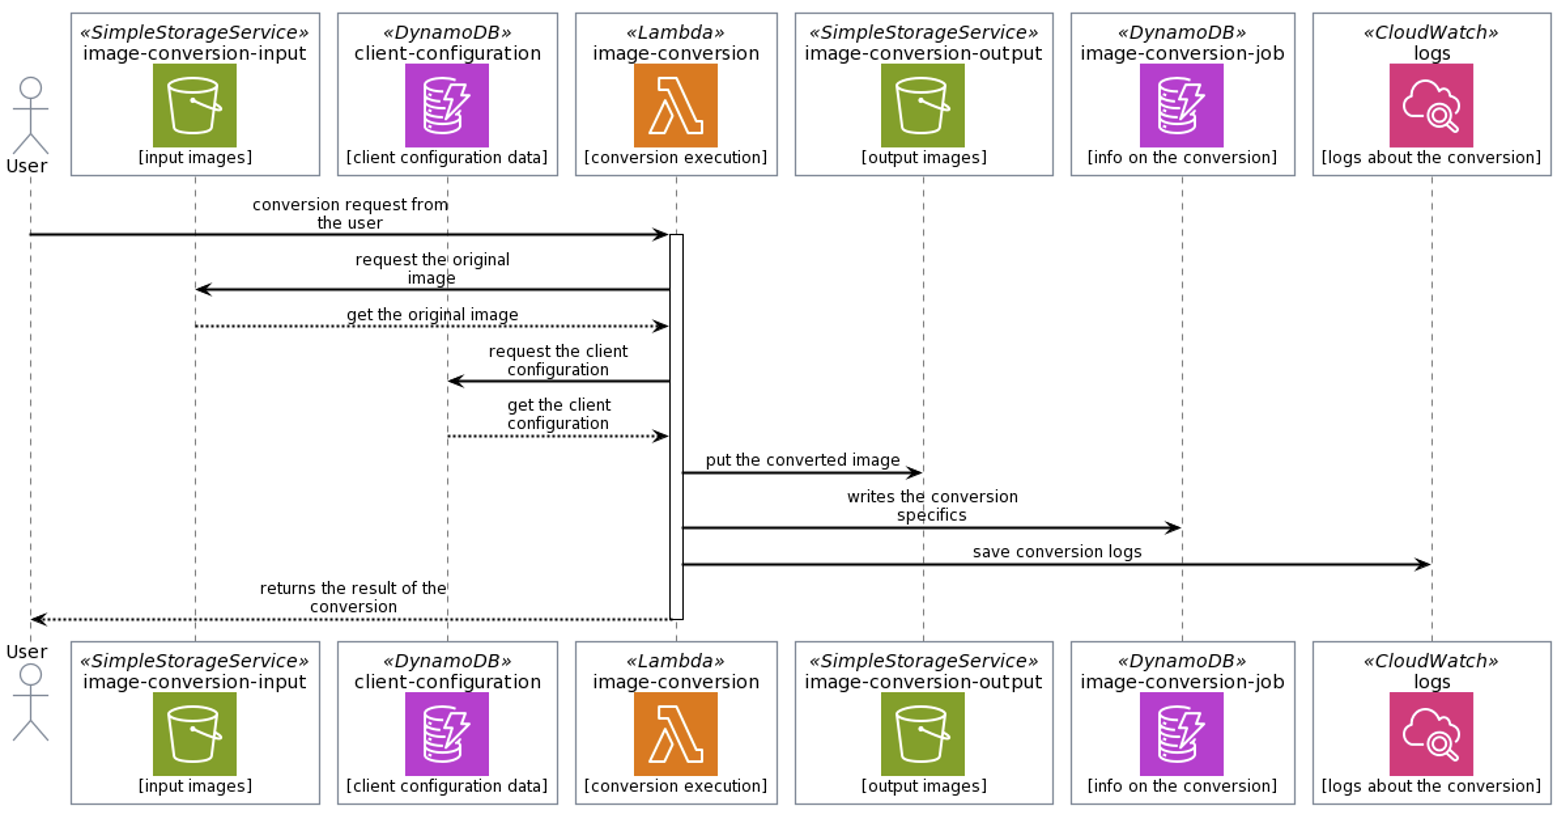
\includegraphics[width=1\textwidth]{images/diagramma-flusso.png}
      \caption{Diagramma di flusso del sistema}
      \label{fig:diagramma-flusso}
\end{figure}

\subsection{Confronto con l'architettura precedente}

Essendo il progetto di stage destinato alla sostituzione di un servizio
attualmente in produzione, è stato necessario confrontare l'architettura
esistente con quella proposta. Le principali differenze sono le seguenti:
\begin{itemize}
      \item \textbf{\emph{deprecazione delle step-function:}} il servizio attuale
            prevede l'utilizzo di \emph{AWS Step Functions}, un servizio che si occupa
            di orchestrare i servizi ad esso legati. L'implementazione di questo
            servizio viene realizzata tramite una macchina a stati, che gestisce il
            flusso di esecuzione in base agli eventi ricevuti. Tra gli eventi
            ricevuti si evidenzia la presenza di una chiamata che permette di
            pulire dall' \glsfirstoccur\gls{EFS} (\emph{Elastic File System}) le
            immagini convertite. \\
            Nel progetto di stage è stato deciso di rimuovere l'utilizzo delle
            \emph{step-functions} per semplificare il flusso della conversione e
            rendere il sistema più semplice da mantenere e da migliorare;
      \item \textbf{\emph{deprecazione dell'EFS:}} il servizio attuale prevede
            l'utilizzo di \emph{EFS} per gestire le immagini da convertire e le
            immagini convertite. \\
            Nel progetto di stage è stato deciso di rimuovere l'utilizzo di \emph{EFS}, in
            quanto la responsabilità della gestione dell'immagine in ambiente
            \emph{serverless} viene delegata completamente al processo eseguito
            dalla \emph{Lambda}, ed eventuali file temporanei non devono più
            essere gestiti manualmente.
\end{itemize}

Queste scelte architetturali portano tuttavia ad una limitazione rispetto al servizio
attualmente in uso, ovvero l'impossibilità di assegnare manualmente la memoria
\emph{RAM} al servizio di conversione. Questa limitazione è dovuta al fatto che
la funzione \emph{Lambda} ha una capacità di memoria massima pari a 10240
\emph{MB}, impedendo l'eventuale conversione di immagini con un peso
superiore.\\
Questa è considerata una limitazione facilmente superabile per due motivi:
\begin{itemize}
      \item il limite di memoria utilizzabile dalla funzione \emph{Lambda} può essere
            contrattato con \emph{AWS}, nel caso vi fosse la necessità di gestire immagini
            con peso superiore al limite attuale;
      \item secondo una analisi delle conversioni effettuate dal servizio attuale,
            prendendo in considerazione tutte le immagini caricate nella piattaforma
            durante il mese di settembre 2023, è stato identificato che il peso medio di
            un'immagine equivale a 9,02 \emph{MB}, con un peso massimo raggiunto di 2,03
            \emph{GB}: entrambe le dimensioni sono ampiamente al di sotto della quota di
            memoria prevista per la funzione \emph{Lambda}.
\end{itemize}



\chapter{Codifica}
\label{cap:codifica}

\intro{Breve introduzione al capitolo}\\

\section{Tecnologie e strumenti}
\label{sec:tecnologie-strumenti}

Di seguito viene data una panoramica delle tecnologie e strumenti utilizzati.

\subsection*{Tecnologia 1}
Descrizione Tecnologia 1.

\subsection*{Tecnologia 2}
Descrizione Tecnologia 2

\section{Ciclo di vita del software}
\label{sec:ciclo-vita-software}

\section{Progettazione}
\label{sec:progettazione}

\subsubsection{Namespace 1} %**************************
Descrizione namespace 1.

\begin{namespacedesc}
    \classdesc{Classe 1}{Descrizione classe 1}
    \classdesc{Classe 2}{Descrizione classe 2}
\end{namespacedesc}


\section{Design Pattern utilizzati}

\section{Codifica}

\chapter{Verifica e validazione}
\label{cap:verifica-validazione}

\intro{In questo capitolo verranno descritte le attività di verifica e
    validazione del prodotto. In particolare verranno descritti i test di unità e di
    sistema, i risultati ottenuti ed eventuali migliorie future da applicare al
    prodotto.}

\section{Test di unità}

Uno dei requisiti fondamentali da soddisfare durante il progetto di stage è
quello riguardante la scrittura di test durante lo sviluppo del codice. In
questa sezione verranno descritti i test di unità, effettuati al fine di
verificare che le singole componenti del sistema funzionassero nella maniera prevista. \\
All'interno del codice, sia nei test, sia nel codice effettivo, sono state
inserite delle variabili d'ambiente che permettono di sostituire il percorso
legato ai profili colore utilizzati: così facendo si ha la possibilità di
eseguire i test anche in locale, senza dover necessariamente effettuare il
\emph{deploy} per verificare che tutto funzioni correttamente.\\
Ogni test di unità è contraddistinto da un codice identificativo, che segue la
seguente nomenclatura: \\
\begin{center}
    \textbf{TU[Codice]}
\end{center}
dove:
\begin{itemize}
    \item \textbf{TU:} definisce che il test è di unità;
    \item \textbf{Codice:} definisce il numero progressivo che contraddistingue il test.
\end{itemize}

Ad ogni test viene assegnato un esito, che può essere di due tipi:
\begin{itemize}
    \item \textbf{S:} il test è stato superato con successo;
    \item \textbf{NS:} il test non è stato superato.
\end{itemize}

Le seguenti tabelle \ref{tab:test-conversioni} e \ref{tab:test-dao} riportano la
lista dei test effettuati per le componenti del sistema, nello specifico quelle
riguardanti le conversioni e quelle riguardanti i \emph{DAO}.
\begin{table}[H]
    \caption{Tabella di tracciamento dei test di unità riguardanti le varie conversioni}
    \label{tab:test-conversioni}
    \centering
    \begin{tabularx}{\textwidth}{|c|c|X|c|}
        \hline
        \textbf{Codice}                  & \textbf{Oggetto} & \textbf{Descrizione}                                                                                                                                                                             & \textbf{Esito} \\
        \hline
        \verb|TU1|                       & VipsConversion   & Verifica del corretto funzionamento della conversione via libreria \emph{vips}, controllando che venisse impostata la risoluzione, il profilo colore, la qualità e il formato desiderati         & S              \\
        \hline
        \verb|TU2|                       & PSDConversion    & Verifica del corretto funzionamento
        della conversione via libreria \emph{go-psd}, controllando che venisse
        impostata la risoluzione desiderata senza
        alterare il rapporto prospettico & S                                                                                                                                                                                                                                    \\
        \hline
        \verb|TU3|                       & EPSConversion    & Verifica del corretto funzionamento della conversione via programma \emph{GhostScript}, controllando che venisse impostata la risoluzione desiderata                                             & S              \\
        \hline
        \verb|TU4|                       & RAWConversion    & Verifica del corretto funzionamento della conversione via programma \emph{Darktable}, controllando che venissero impostate la risoluzione, il profilo colore, la qualità e il formato desiderati & S              \\
        \hline
    \end{tabularx}
\end{table}

\begin{table}[H]
    \caption{Tabella di tracciamento dei test di unità riguardanti i \emph{DAO}}
    \label{tab:test-dao}
    \begin{tabularx}{\textwidth}{|c|c|X|c|}
        \hline
        \textbf{Codice}                                          &
        \textbf{Oggetto}                                         & \textbf{Descrizione }  & \textbf{Esito} \\
        \hline
        \verb|TU5|                                               & ClientConfigurationDAO & Verifica del
        corretto funzionamento del \emph{DAO} che ritorna la configurazione del
        cliente specificato                                      & S                                       \\
        \hline
        \verb|TU6|                                               & ConversionsBucketDAO   & Verifica del
        corretto funzionamento del \emph{DAO} che si occupa di effettuare il
        caricamento e il salvataggio dei file su \emph{S3}       & S                                       \\
        \hline
        \verb|TU7|                                               & ImageConversionJobsDAO & Verifica del
        corretto funzionamento del \emph{DAO} che si occupa di inserire ed
        effettuare l'aggiornamento dei \emph{job} di conversione & S                                       \\
        \hline
    \end{tabularx}
\end{table}

I test effettuati sono stati utili per mostrare lacune ed errori nel codice
scritto. Il codice delle funzioni testate non ha funzionato al primo tentativo,
ed è stato necessario riscrivere più volte le funzioni per ottenere il risultato
desiderato. \\
La scrittura dei test, in generale, è risultata semplice ed intuitiva: ho
utilizzato anche una caratteristica del linguaggio \emph{Go}, ossia i test
\emph{table-driven}: è possibile specificare una tabella di test per eseguire
più volte una stessa porzione di codice, con input differenti. Questo è
risultato molto utile per testare più agevolmente le multiple combinazioni di
conversioni possibili.

\section{Test di sistema}

In questa sezione vengono descritti i test di sistema effettuati sul progetto di
stage. Questi test hanno lo scopo di verificare il corretto funzionamento del
codice con tutti i formati di immagine supportati e con diverse configurazioni
per singolo cliente. Durante questo test viene verificato anche se i \emph{DAO}
funzionano correttamente, in quanto è stato replicato il funzionamento completo
del servizio. \\
Per effettuare la fase di test in locale, sono state necessarie diverse
componenti e software aggiuntivi, che ora andrò ad elencare:
\begin{itemize}
    \item \textbf{Immagini di test:} queste immagini venivano recuperate da una
          cartella denominata \emph{test-images}, in cui era presente un'immagine per
          ogni formato supportato e previsto dai requisiti funzionali;
    \item \textbf{Localstack:} è un \emph{framework} che permette di emulare
          alcuni servizi \emph{AWS} in locale, tra cui \emph{S3}. Questo servizio viene lanciato da uno script
          \glsfirstoccur\gls{bash}, che si occupa di creare i due \emph{bucket}
          necessari per l'\emph{upload} e il \emph{download} delle immagini; \cite{localstack}
    \item \textbf{Docker e docker-compose:} sono due strumenti che hanno
          permesso di creare in modo semplice e veloce un \emph{container} in cui
          creare due istanze di \emph{DynamoDB}, al fine di ricreare le tabelle della
          configurazione e dei \emph{job} di conversione. I database vengono creati a
          grazie ad un comando \emph{bash} che si occupa di lanciare il
          \emph{container} e creare le risorse seguendo il modello specificato nel
          file di infrastruttura del codice. Con \emph{Docker} è stato creato
          anche un \emph{container} su cui viene lanciata la \emph{Lambda}
          direttamente da riga di comando, solo dopo avere inserito le
          credenziali di accesso all'ambiente \emph{sandbox};
    \item \textbf{File JSON di configurazione:} è stato creato un file di tipo
          \emph{JSON} in cui sono state contenute alcune configurazioni di test per il
          cliente \emph{test-client}. Nello specifico le configurazioni sono state le
          seguenti:
          \begin{itemize}
              \item \textbf{Configurazione "ORIGINAL":} larghezza impostata a $0$,
                    altezza impostata a $0$, qualità impostata a $100$. Si è deciso di
                    utilizzare come valore sentinella lo $0$, così da poter verificare che
                    venissero utilizzate le dimensioni originali dell'immagine in ingresso
                    per la conversione;
              \item \textbf{Confiurazione "4K":} larghezza impostata a $3840$, altezza
                    impostata a $2160$, qualità impostata a $100$;
              \item \textbf{Configurazione "2K":} larghezza impostata a $2560$, altezza
                    impostata a $1440$, qualità impostata a $100$;
              \item \textbf{Configurazione "FULLHD":} larghezza impostata a $1920$,
                    altezza impostata a $1080$, qualità impostata a $100$;
              \item \textbf{Configurazione "HD":} larghezza impostata a $1280$, altezza
                    impostata a $720$, qualità impostata a $100$;
          \end{itemize}
\end{itemize}

Ogni test di sistema è contraddistinto da un codice identificativo, che segue la
seguente nomenclatura: \\
\begin{center}
    \textbf{TS[Codice]}
\end{center}
dove:
\begin{itemize}
    \item \textbf{TS:} definisce che il test è di sistema;
    \item \textbf{Codice:} definisce il numero progressivo che contraddistingue il test.
\end{itemize}

Di seguito viene riportata la tabella \ref{tab:test-sistema} che riporta i test
di sistema effettuati sul progetto di stage.

\begin{table}[H]
    \caption{Tabella di tracciamento dei test di sistema}
    \label{tab:test-sistema}
    \begin{tabularx}{\textwidth}{|c|c|X|c|}
        \hline
        \textbf{Codice}                                      & \textbf{Oggetto} & \textbf{Descrizione}                           & \textbf{Esito} \\
        \hline
        \verb|TS1|                                           & Conversione      & Verifica del corretto funzionamento
        del servizio di conversione per ogni immagine, verificando che la stessa
        venga convertita correttamente, seguendo la configurazione recuperata e
        impedendo la conversione in caso di \emph{upscaling} & S
        \\
        \hline
        \verb|TS2|                                           & DAO              & Verifica del corretto funzionamento di tutti i
        DAO, controllando che venga eseguito il recupero della configurazione della
        conversione, che venga effettuato il \emph{download} dell'immagine da
        convertire e che venga caricata nel \emph{bucket} di destinazione al termine
                                                             & S
        \\
        \hline
    \end{tabularx}
\end{table}

\section{Documentazione}

Un obiettivo obbligatorio previsto dal progetto di stage è stato quello di redigere la
documentazione sul progetto svolto, di tipo funzionale e tecnico. La prima delle
due è stata realizzata per descrivere il funzionamento del servizio a tutto il
team \emph{Contenuti}, fornendo informazioni utili a seguire il flusso della
conversione e per fornire una guida su come viene utilizzato il servizio. La documentazione tecnica invece pone l'attenzione sui dettagli
implementativi del codice ed è stata realizzata per fornire informazioni
riguardanti il codice e le tecnologie utilizzate per chi lavora nel lato \emph{back-end} del team: così facendo chiunque si troverà a
lavorare sul progetto potrà farlo in autonomia.\\
La documentazione è stata validata dal tutor aziendale, che ha accompagnato il
processo di stesura fornendo \emph{feedback} sulle parti da migliorare e
approfondire, man mano che venivano implementate nuove funzionalità. \\
Di seguito vengono descritte nel dettaglio le due tipologie di documentazione:
\begin{itemize}
    \item \textbf{Documentazione funzionale:} la documentazione funzionale è
          stata scritta in modo da essere comprensibile anche a chi non ha esperienza
          tecnica sul progetto. Viene infatti fornita una panoramica generale del
          servizio, elencandone le funzionalità ad alto livello ed il flusso di
          conversione seguito.
    \item \textbf{Documentazione tecnica:} la documentazione tecnica presenta
          tutte le informazioni necessarie per poter lavorare sul progetto in
          maniera autonoma, fornendo le informazioni riguardanti i comandi per
          installare gli applicativi e le librerie necessarie al corretto
          funzionamento del servizio. Sono presenti anche i comandi per
          effettuare la validazione dello \emph{stack} di risorse definito e per
          effettuare il \emph{deploy}. \\
          Vengono elencati i comandi per preparare l'ambiente di test in
          locale, fornendo una guida su come eseguire i \emph{container} che
          raccolgono i servizi \emph{AWS} emulati, e vengono fornite
          informazioni su come poter eseguire una dimostrazione del servizio,
          lanciando la \emph{Lambda} da riga di comando con una serie di
          conversioni di test.
\end{itemize}

Entrambe le documentazioni sono state inserite nel file \emph{README} presente
all'interno del progetto, così da essere sempre disponibile durante il lavoro
sul codice.

\section{Collaudo}

Durante il periodo di stage, sono stati previsti dei momenti di verifica
informale con il tutor aziendale, al fine di mostrare i progressi ottenuti sul
progetto e per ricevere \emph{feedback} sulle funzionalità implementate. Durante
le fasi di sviluppo sono state effettuate delle \glsfirstoccur\gls{pull-request}
su \emph{CodeCommit}, così da poter mantenere una versione stabile del progetto
nel ramo \emph{main} del repository ed avere una versione dove poter integrare
tutte le nuove funzionalità nel ramo \emph{dev}. Le funzionalità del ramo
\emph{dev} considerate stabili dovevano essere sottoposte al processo di
\glsfirstoccur\gls{code-review} da parte del tutor aziendale, al fine di
garantire che venissero implementate sempre nel modo corretto, fornendo
\emph{feedback} su eventuali errori presenti nel codice.

\section{Presentazione finale}

Nell'ultimo giorno di stage è stata effettuata la presentazione finale del
progetto, permettendomi di mostrare il lavoro svolto durante il periodo di stage
e i risultati ottenuti. La presentazione si è svolta davanti a tutta l'azienda,
al fine di fornire una panoramica generale del progetto a tutti i dipendenti. \\
L'esito della presentazione è stato decisamente positivo e le domande poste dai
presenti non hanno evidenziato critcità sul progetto ma hanno offerto alcuni
spunti per eventuali migliorie future.\\
La presentazione è stata una validazione ad alto livello del lavoro svolto
durante il periodo di stage.

\section{Migliorie future}
Al termine dell'attività di stage sono state individuate alcune possibili
migliorie future, per ampliare il servizio e fornire maggiori funzionalità. \\
Sono stati individuati i seguenti possbili miglioramenti:
\begin{itemize}
    \item \textbf{Implementazione di una \emph{dashboard} su \emph{CloudWatch}:}
          attualmente il servizio permette il recupero di informazioni legate al
          servizio solo tramite \emph{query} al database \emph{DynamoDB}. Per ovviare
          a ciò sarebbe possibile definire una \emph{dashboard} su \emph{CloudWatch},
          che possa offrire una rappresentazione visiva più efficace delle metriche legate al
          funzionamento del servizio. Tale \emph{dashboard} può essere utilizzata dal
          reparto tecnico per ottenere informazioni specifiche su aspetti essenziali
          della conversione, quali la durata minima, media e massima di elaborazione o
          anche la dimensione minima, media e massima dei file gestiti dal servizio;
    \item \textbf{Implementazione di una \emph{API} per leggere i \emph{job}
              salvati:} attualmente il servizio permette di recuperare i \emph{job} di
          conversione salvati tramite \emph{query} al database \emph{DynamoDB}. Al
          fine di poter recuperare in maniera più semplice e veloce tali informazioni,
          si potrebbe implementare una \emph{API} che permetta di recuperare i
          \emph{job} salvati, restituendoli nella console amministrativa interna dell'azienda.
\end{itemize}

\section{Consuntivo finale}

Di seguito viene riportato il diagramma di Gantt, aggiornato con le attività
svolte.

\begin{figure}[H]
    \centering
    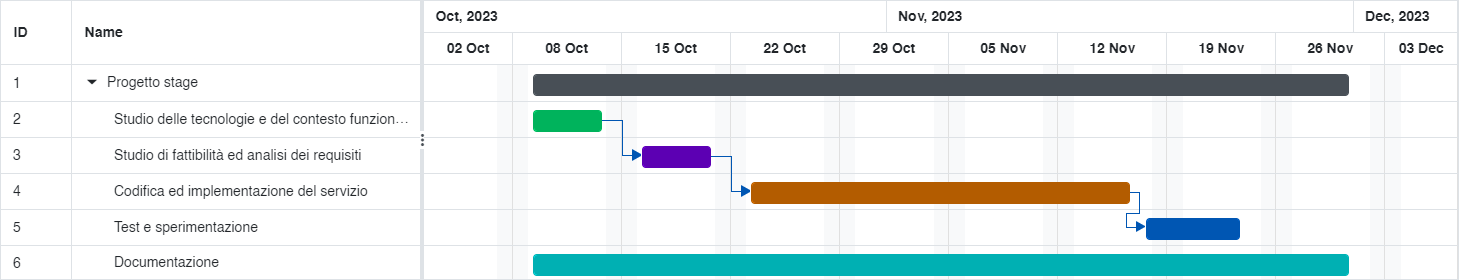
\includegraphics[width=\textwidth]{images/gantt.png}
    \caption{Diagramma di Gantt aggiornato con le attività svolte}
    \label{fig:gantt-finale}
\end{figure}

Di seguito vengono specificate le ore impiegate per ogni fase del progetto:
\begin{itemize}
    \item \textbf{Studio delle teconologie e del contesto funzionale:} per lo
          studio delle tecnologie da utilizzare sono state impiegate $40$ ore, in
          linea con il piano di lavoro iniziale;
    \item \textbf{Studio di fattibilità e analisi dei requisiti:} per effettuare
          l'analisi dei requisiti e lo studio di fattibilità sono state impiegate
          $40$ ore, in linea con quanto previsto dal piano di lavoro;
    \item \textbf{Codifica ed implementazione del servizio:} per la fase di
          codifica del servizio sono state impiegate $150$ ore, $30$ in più rispetto a
          quelle previste dal piano iniziale. Questo è dovuto al fatto che è stato
          speso molto più tempo nella fase di codifica della \emph{Proof of Concept},
          risultata poi fondamentale per lo sviluppo del servizio, in quanto ha
          permesso di accelerare di molto la fase di sviluppo del servizio in ambiente
          \emph{serverless};
    \item \textbf{Test e sperimentazione:} per la fase di test e sperimentazione
          sono state impiegate $34$ ore, $46$ in meno rispetto a quelle
          preventivate. Il motivo di tale discrepanza è dovuto a due aspetti: il primo
          riguarda i test, che sono stati scritti man mano che venivano sviluppate le
          funzionalità del servizio e ciò ha permesso di recuperare tempo che è stato
          impiegato nella fase di codifica per ottenere un codice più stabile. Il
          secondo aspetto riguarda la sperimentazione, che è stata fatta in maniera
          meno approfondita, preferendo la pulizia e la stabilità del codice scritto.
    \item \textbf{Documentazione:} per la fase di scrittura della documentazione
          sono state impiegate $40$ ore, in linea rispetto a quanto previsto nel piano
          di lavoro iniziale.
\end{itemize}

In totale sono state impiegate $304$ ore per il progetto di stage, $16$ ore in
meno rispetto alle $320$ previste inizialmente. Questo è da attribuirsi al fatto
che lo stage è terminato il $30/11/2023$, anziché il $01/12/2023$, poichè era
necessario che lo stage fosse terminato prima di tale data, al fine di poter
effettuare correttamente il
riconoscimento dei crediti dell'attività. Inoltre il giorno $01/11/2023$ era un
giorno di festività nazionale, che non è stato considerato nel piano di lavoro.
\chapter{Conclusioni}
\label{cap:conclusioni}



\section{Consuntivo finale}

\section{Raggiungimento degli obiettivi}

\section{Conoscenze acquisite}

\section{Valutazione personale}

\cleardoublepage
\phantomsection
\pdfbookmark{Ringraziamenti}{ringraziamenti}

\begin{flushright}{
    \slshape
    ``Life is really simple, but we insist on making it complicated''} \\
    \medskip
    --- Confucius
\end{flushright}


\bigskip

\begingroup
\let\clearpage\relax
\let\cleardoublepage\relax
\let\cleardoublepage\relax

\chapter*{Ringraziamenti}

\noindent \textit{Innanzitutto, vorrei esprimere la mia gratitudine al Prof. \myProf, relatore della mia tesi, per l'aiuto e il sostegno fornitomi durante la stesura del lavoro.}\\

\noindent \textit{Desidero ringraziare con affetto i miei genitori per il sostegno, il grande aiuto e per essermi stati vicini in ogni momento durante gli anni di studio.}\\

\noindent \textit{Ho desiderio di ringraziare poi i miei amici per tutti i bellissimi anni passati insieme e le mille avventure vissute.}\\
\bigskip

\noindent\textit{\myLocation, \myTime}
\hfill \myName

\endgroup


\appendix

\backmatter
\printglossary[type=main, title=Glossario, toctitle=Glossario]

\cleardoublepage
\chapter{Bibliografia}

\nocite{*}

% Print book bibliography
\printbibliography[heading=subbibliography,title={Riferimenti bibliografici},type=book]

% Print site bibliography
\printbibliography[heading=subbibliography,title={Siti web consultati},type=online]

\end{document}
